% Informe del proyecto CS4052 - Caso 5: KNN en paralelo con MPI.
% Compilar desde esta carpeta:  latexmk -pdf informe.tex
% Las figuras de resultados se generan con src/graficas.py en results/final/figuras.
\documentclass[11pt,a4paper]{article}

\usepackage[utf8]{inputenc}
\usepackage[T1]{fontenc}
\usepackage{lmodern}
\usepackage[spanish,es-tabla,es-nodecimaldot]{babel}
\usepackage[margin=2.4cm]{geometry}
\usepackage{amsmath,amssymb}
\usepackage{booktabs,array,tabularx}
\usepackage{enumitem}
\usepackage{xcolor}
\usepackage{caption}
\usepackage{graphicx}
\graphicspath{{../../results/final/figuras/}}
\usepackage[ruled,vlined,linesnumbered,spanish,onelanguage]{algorithm2e}
\usepackage{tikz}
\usetikzlibrary{babel,arrows.meta,positioning,fit,calc}
\usepackage[hidelinks]{hyperref}

\setlist[itemize]{noitemsep,topsep=3pt}
\captionsetup{font=small}
\setlength{\parskip}{3pt}

% Notación
\newcommand{\ntr}{n_{tr}}
\newcommand{\nte}{n_{te}}
\newcommand{\Xtr}{X_{tr}}
\newcommand{\Xte}{X_{te}}
\newcommand{\ytr}{y_{tr}}
\newcommand{\yte}{y_{te}}
\newcommand{\Tinf}{T_\infty}
\newcommand{\tcomm}[1]{T_{comm_{#1}}}
\newcommand{\tcomp}[1]{T_{comp_{#1}}}

% Palabras clave del pseudocódigo
\SetKwFor{ParaPar}{for}{\textcolor{red}{\textbf{pardo}}}{}
\SetKwFor{Para}{for}{do}{}
\SetKwIF{Si}{SinoSi}{Sino}{if}{then}{else if}{else}{}
\SetKwInput{Entrada}{Entrada}
\SetKwInput{Salida}{Salida}
\SetKwComment{Paso}{// }{}
\SetCommentSty{texttt}
\SetKw{Retorna}{return}
\SetKwFunction{Bcast}{Broadcast}
\SetKwFunction{Scatter}{Scatter}
\SetKwFunction{Gather}{Gather}
\SetKwFunction{Reduce}{Reduce}

\begin{document}

% ---------------------------------------------------------------- Título
\begin{center}
  {\large \textbf{CS4052 Computación Paralela y Distribuida} -- 2026-II}\\[2pt]
  Proyecto de Laboratorio -- \textbf{Entrega final}\\[6pt]
  {\LARGE Caso 5: KNN en paralelo con MPI (mpi4py)}\\[4pt]
  Clasificación de dígitos (\textit{load\_digits})\\[6pt]
  Profesor: José Fiestas \quad -- \quad Grupo 7
\end{center}

\begin{center}
\begin{tabular}{lc}
  \toprule
  \textbf{Integrante} & \textbf{Participación} \\
  \midrule
  Barzola Estrella, Johar Jared   & 100\,\% \\
  Huaman Casma, Leonardo Fabian   & 100\,\% \\
  Izaguirre Zavaleta, Luis Fernando & 100\,\% \\
  \bottomrule
\end{tabular}\\[3pt]
{\small (100\,\% indica que el integrante contribuyó en forma equitativa al resto)}
\end{center}

% ---------------------------------------------------------------- 1
\section{Introducción}

KNN (\textit{k-nearest neighbors}) es un algoritmo de clasificación supervisada. Para clasificar un punto nuevo, calcula su distancia a todos los puntos de entrenamiento, toma los $k$ más cercanos y le asigna la etiqueta que más se repite entre ellos.

En este proyecto paralelizamos el código secuencial \texttt{knn\_digits\_sec.py} \cite{base}, que clasifica las imágenes del conjunto \textit{load\_digits} de scikit-learn \cite{sklearn}. El conjunto tiene $n=1797$ imágenes de $8\times 8$ píxeles, es decir $d=64$ características, y 10 clases. El código separa los datos con \texttt{train\_test\_split} (20\,\% para prueba, \texttt{random\_state=42}), lo que da $\ntr=1437$ puntos de entrenamiento y $\nte=360$ de prueba, y usa $k=3$. Su precisión (\textit{accuracy}) es $0{,}9833$, que tomamos como referencia.

El trabajo más costoso es calcular las $\ntr\cdot\nte$ distancias, y cada una se puede calcular de forma independiente de las demás. Por eso es un problema naturalmente paralelizable \cite{slides}.

\textbf{Solución planteada.} Usamos el paradigma de memoria distribuida (paso de mensajes), en Python con mpi4py \cite{mpi4py}. El proceso 0 (maestro) tiene los datos al inicio. Siguiendo el DAG del enunciado \cite{enunciado} (Figura~\ref{fig:dag}):
\begin{itemize}
  \item se envían los datos de prueba a todos los procesos (\texttt{comm.bcast});
  \item se reparten los datos de entrenamiento en bloques (\texttt{comm.scatter});
  \item cada proceso calcula las distancias de todos los puntos de prueba a su bloque, las ordena y guarda sus $k$ vecinos más cercanos por punto de prueba;
  \item el maestro recolecta esos candidatos (\texttt{comm.gather}), elige los $k$ más cercanos de todos y aplica la votación por mayoría.
\end{itemize}

Si un punto es uno de los $k$ vecinos más cercanos entre todos los datos de entrenamiento, también lo es dentro de su bloque: de lo contrario, ese bloque tendría al menos $k$ puntos más cercanos, y el punto no podría ser vecino global. Por ello, al reunir los candidatos locales y seleccionar otra vez los $k$ de menor distancia, se recuperan los mismos vecinos del algoritmo secuencial, salvo empates de distancia.

Para preparar este informe usamos un asistente de IA \cite{ia}; en la Bibliografía describimos para qué lo usamos y en qué partes influyó.

\begin{figure}[ht]
\centering
\begin{tikzpicture}[
  nodo/.style={circle,draw,thick,minimum size=14mm,align=center,font=\scriptsize,inner sep=1pt},
  flecha/.style={-{Stealth[length=2.5mm]},thick},
  com/.style={font=\scriptsize,text=blue!70!black},
  cmp/.style={font=\scriptsize,text=red!75!black}]
  \node[nodo] (ini) at (0,3.6) {Datos\\iniciales};
  \node[nodo] (p0) at (-3,0) {dist\\sort\\k-nearest};
  \node[nodo] (p1) at (-1,0) {dist\\sort\\k-nearest};
  \node at (1,0) {$\cdots$};
  \node[nodo] (pp) at (3,0) {dist\\sort\\k-nearest};
  \node[nodo] (fin) at (0,-3.6) {selección\\y votación};
  \foreach \x in {p0,p1,pp} {
    \draw[flecha] (ini) -- (\x);
    \draw[flecha] (\x) -- (fin);
  }
  \node[com,anchor=east] at (-2.0,2.45) {Scatter: $O\big(\log p\,(a+\tfrac{\ntr}{p}\, b)\big)$};
  \node[com,anchor=west] at (2.0,2.45) {Broadcast: $O\big(\log p\,(a+\nte\, b)\big)$};
  \node[cmp,anchor=east] at (-3.9,0) {$O(\ntr\,\nte/p)$};
  \node[com,anchor=east] at (-2.0,-2.45) {Gather: $O\big(\log p\,(a+\nte\,k\,b)\big)$};
  \node[cmp,anchor=west] at (1.0,-3.6) {$O(\nte\,p\,k)$};
\end{tikzpicture}
\caption{DAG del KNN en paralelo, adaptado de \cite{enunciado} con los costos de \texttt{scatter} y \texttt{gather} corregidos a $O(\log p)$ (Sección~\ref{sec:metricas}), confirmado por el profesor \cite{slides,correo-profesor}. En azul, comunicación; en rojo, cómputo. Aquí $\nte$ cuenta puntos, con $d$ constante.}
\label{fig:dag}
\end{figure}

% ---------------------------------------------------------------- 2
\section{Método}

\subsection{Algoritmo secuencial}
\label{sec:secuencial}

Llamamos $n=\ntr+\nte$ al tamaño de los datos. La división 80/20 se mantiene fija, así que $\nte=c\,n$ y $\ntr=(1-c)\,n$ con $c\approx 0{,}2$. Con esto, el problema depende de un \textbf{solo tamaño} $n$, y $\ntr\,\nte=c(1-c)\,n^2\approx 0{,}16\,n^2$. El tiempo secuencial se obtiene del código base \cite{base} (Tabla~\ref{tab:secuencial}).

\begin{table}[ht]
\centering\footnotesize
\begin{tabular}{ll}
  \toprule
  \textbf{Línea del código secuencial} & \textbf{Operaciones} \\
  \midrule
  \texttt{euclidean\_distance(a, b)} & $d$ restas, $d$ productos, $d-1$ sumas y 1 raíz: $O(d)$ \\
  \texttt{distances = [... for x in X\_train]} & $\ntr\cdot O(d)$ \\
  \texttt{np.argsort(distances)[:k]} & $O(\ntr\log\ntr)$ \\
  \texttt{k\_labels = [y\_train[i] for i in k\_indices]} & $O(k)$ \\
  \texttt{Counter(k\_labels).most\_common(1)} & $O(k)$ \\
  \texttt{y\_pred = [knn\_predict(x, ...) for x in X\_test]} & lo anterior se repite $\nte$ veces \\
  \texttt{accuracy = np.mean(y\_pred == y\_test)} & $O(\nte)$, una sola vez \\
  \bottomrule
\end{tabular}
\caption{Operaciones de cada línea del código secuencial \cite{base}.}
\label{tab:secuencial}
\end{table}

\[
T_s(n)=O\big(\nte(\ntr\, d+\ntr\log\ntr+k)+\nte\big)=O\big(n^2(d+\log n)\big)
\]
Como $d=64>\log_2 n\approx 10{,}8$, el cálculo de distancias domina al ordenamiento:
\[
T_s(n)=O(d\,n^2)
\]

\subsection{Diseño con el método de Foster}
\label{sec:foster}

La Figura~\ref{fig:foster} resume los cuatro pasos de Foster \cite{slides}.

\textbf{Particionamiento.} Usamos descomposición del dominio sobre la data de mayor tamaño, la de entrenamiento ($\ntr>\nte$). La tarea primitiva es la distancia entre un punto de prueba y uno de entrenamiento, lo que da $\ntr\cdot\nte=517\,320$ tareas de costo $O(d)$ y de tamaño parecido, más de cuatro órdenes de magnitud por encima de $p=16$ \cite{slides}.

\textbf{Comunicación.} Cada tarea necesita sus dos puntos, y su distancia se usa luego para elegir los $k$ vecinos de ese punto de prueba. Es decir, las tareas de una misma fila se combinan en una reducción. Contando solo las salidas, son del orden de $\ntr\,\nte\approx 5{,}2\times 10^5$ canales hacia la selección. Esta comunicación es \textit{overhead}: no existe en el secuencial.

\textbf{Aglomeración.} Agrupamos en una tarea todas las columnas de un bloque de puntos de entrenamiento. Así, cada proceso recibe solo su bloque y los datos de prueba, y envía $k$ candidatos por punto de prueba en lugar de todas sus distancias. Contando un canal de Broadcast, uno de Scatter y uno de Gather por bloque, quedan del orden de $3p$ canales.

\textbf{Mapeo.} Asignamos un bloque por proceso. Como $\ntr=1437$ no es múltiplo de $p$ para $p=2,4,8,16$, los primeros $\ntr \bmod p$ procesos reciben $\lceil\ntr/p\rceil$ puntos y el resto $\lfloor\ntr/p\rfloor$. Los bloques difieren en un punto como máximo, así que la carga queda balanceada y en el análisis usamos $\ntr/p$ \cite{slides}. Con $p=16$ son unos 48 canales.

\begin{figure}[ht]
\centering
\begin{tikzpicture}[
  scale=0.42,
  tarea/.style={circle,fill=black!60,inner sep=0pt,minimum size=1.6mm},
  titulo/.style={font=\footnotesize\bfseries,anchor=south},
  flecha/.style={-{Stealth[length=2mm]},thick},
  every node/.append style={font=\scriptsize}]
  % 1. Particionamiento
  \begin{scope}
    \foreach \i in {0,...,3} \foreach \j in {0,...,5} \node[tarea] at (\j,\i) {};
    \node[titulo] at (2.5,4.1) {1. Particionamiento};
    \node at (2.5,-1.1) {$\ntr$ (columnas)};
    \node[rotate=90] at (-1.1,1.5) {$\nte$ (filas)};
  \end{scope}
  % 2. Comunicación
  \begin{scope}[xshift=9.3cm]
    \foreach \i in {0,...,3} {
      \draw[blue!70!black,thick] (0,\i) -- (5,\i);
      \foreach \j in {0,...,5} \node[tarea] at (\j,\i) {};
    }
    \node[titulo] at (2.5,4.1) {2. Comunicación};
    \node at (2.5,-1.1) {reducción por fila};
  \end{scope}
  % 3. Aglomeración
  \begin{scope}[xshift=18.6cm]
    \foreach \i in {0,...,3} \foreach \j in {0,...,5} \node[tarea] at (\j,\i) {};
    \foreach \x/\c in {0/orange,2/teal,4/violet}
      \draw[\c,very thick,rounded corners=2pt,fill=\c,fill opacity=0.15]
        (\x-0.4,-0.4) rectangle (\x+1.4,3.4);
    \node[titulo] at (2.5,4.1) {3. Aglomeración};
    \node at (2.5,-1.1) {bloques de $\ntr/p$};
  \end{scope}
  % 4. Mapeo
  \begin{scope}[xshift=27.9cm]
    \foreach \x/\c/\t in {0/orange/$P_0$,2/teal/$P_1$,4/violet/$P_{p-1}$} {
      \draw[\c,very thick,rounded corners=2pt,fill=\c,fill opacity=0.15]
        (\x-0.4,1.4) rectangle (\x+1.4,3.4);
      \node[text opacity=1] at (\x+0.5,2.4) {\t};
      \draw[flecha,black!70] (\x+0.5,1.3) -- (2.5,0.5);
    }
    \node[draw,thick,rounded corners=2pt,inner sep=2pt] at (2.5,0) {votación};
    \node[titulo] at (2.5,4.1) {4. Mapeo};
    \node at (2.5,-1.1) {un bloque por proceso};
  \end{scope}
\end{tikzpicture}
\caption{Método de Foster aplicado al KNN. Cada punto es una distancia entre un punto de prueba y uno de entrenamiento.}
\label{fig:foster}
\end{figure}

El enunciado también menciona repartir los datos de prueba. Esa alternativa (\textit{scatter} de prueba y \textit{broadcast} de entrenamiento) es válida y evita el paso 6 en el maestro. Sin embargo, seguimos la distribución del DAG, que reparte el conjunto de mayor tamaño.

\subsection{PRAM}
\label{sec:pram}

El Algoritmo~\ref{alg:knn} presenta el pseudocódigo con la notación PRAM del curso \cite{slides,pd02}. No depende de $p$: los límites de los bucles se expresan solo con el tamaño del problema, y \textbf{pardo} va en el bucle sobre $\ntr$, que es la dimensión que se distribuye. El número de procesos aparece recién al ejecutar ese \textbf{pardo}, cuando cada proceso toma un bloque de valores de $j$ y aplica la línea 6 solo a ellos; por eso el Gather reúne varias listas de candidatos por punto de prueba. Esto permite leer directamente el trabajo $W$ y el \textit{span} $\Tinf$ (Sección~\ref{sec:span}).

\begin{algorithm}[ht]
\caption{KNN distribuido con Broadcast/Scatter/Gather$(\Xtr,\ytr,\Xte,\yte,k)$}
\label{alg:knn}
\DontPrintSemicolon
\Entrada{datos de entrenamiento $\Xtr$ ($\ntr\times d$) con etiquetas $\ytr$; datos de prueba $\Xte$ ($\nte\times d$) con etiquetas $\yte$; $k$ vecinos}
\Salida{etiquetas predichas $\hat y[1,\dots,\nte]$ y precisión en el proceso raíz}
\Bcast{$\Xte,k,root=0$}\Paso*[r]{paso 1}
\Scatter{$(\Xtr,\ytr),root=0$}\Paso*[r]{paso 2}
\Para{$i\gets 1$ \KwTo $\nte$}{
  \ParaPar{$j\gets 1$ \KwTo $\ntr$}{
    $D[j]\gets\sqrt{\sum_{l=1}^{d}\big(\Xte[i,l]-\Xtr[j,l]\big)^2}$\Paso*[r]{paso 3}
  }
  $L[i]\gets$ los $k$ pares $(D[j],\ytr[j])$ de menor distancia\Paso*[r]{paso 4}
}
\Gather{$L,C,root=0$}\Paso*[r]{paso 5}
\Si{es el proceso raíz}{
  \Para{$i\gets 1$ \KwTo $\nte$}{
    $V\gets$ los $k$ pares de menor distancia en $C[i]$\Paso*[r]{paso 6}
    $\hat y[i]\gets$ etiqueta más frecuente en $V$\;
  }
  $accuracy\gets$ (cantidad de $i$ con $\hat y[i]=\yte[i]$) $/\ \nte$\Paso*[r]{paso 7}
  \Retorna{$\hat y,accuracy$}\;
}
\end{algorithm}

\textbf{Descripción de los pasos:}
\begin{itemize}
  \item \textbf{Paso 1:} el maestro envía los $\nte$ datos de prueba y $k$ a todos los procesos.
  \item \textbf{Paso 2:} el maestro reparte los datos de entrenamiento y sus etiquetas en bloques.
  \item \textbf{Paso 3:} se calculan las distancias de cada punto de prueba a los puntos de entrenamiento. Cada proceso calcula las de su bloque.
  \item \textbf{Paso 4:} por cada punto de prueba, cada proceso ordena las distancias de su bloque y guarda sus $k$ vecinos locales (distancia y etiqueta).
  \item \textbf{Paso 5:} el maestro recolecta en un solo \texttt{Gather} los candidatos de todos los puntos de prueba, para no pagar la latencia $\nte$ veces.
  \item \textbf{Paso 6:} por cada punto de prueba, el maestro elige los $k$ pares de menor distancia entre todos los candidatos y aplica la votación. No se debe votar directamente con todos los candidatos: se votaría con más de $k$ vecinos y el resultado podría diferir del secuencial.
  \item \textbf{Paso 7:} el maestro calcula la precisión comparando $\hat y$ con $\yte$.
\end{itemize}

Si lo vemos como un PRAM de memoria compartida, el algoritmo es CREW \cite{slides}: todos leen $\Xte$ al mismo tiempo y cada uno escribe solo en sus posiciones. En memoria distribuida, la lectura concurrente se reemplaza por el Broadcast del paso 1.

\subsubsection*{Optimización del paso 6}

En el Algoritmo~\ref{alg:knn}, el maestro hace solo todo el paso 6 y recibe todos los candidatos. Ambos costos crecen con $p$. Podemos evitarlo porque elegir los $k$ menores es una operación asociativa: si $A\oplus B$ denota los $k$ pares de menor distancia de $A\cup B$, entonces $(A\oplus B)\oplus C=A\oplus(B\oplus C)$. A diferencia de una suma \cite{slides}, $\oplus$ no cuesta tiempo constante, sino $O(k)$ por punto de prueba; como $k$ es constante, la cota no cambia. Así, la selección se puede hacer como una \textbf{reducción en árbol}, en la que cada nivel fusiona listas de $k$ pares y solo reenvía $k$ pares por punto de prueba. El Algoritmo~\ref{alg:knnred} reemplaza las líneas 7 a 11 del Algoritmo~\ref{alg:knn}; las líneas 12 y 13 no cambian. En mpi4py corresponde a \texttt{comm.reduce} con una operación propia, que para objetos de Python usa una reducción en árbol por defecto \cite{mpi4py}.

\begin{algorithm}[ht]
\caption{Pasos 5 y 6 optimizados con una reducción en árbol}
\label{alg:knnred}
\DontPrintSemicolon
\Reduce{$L,C,op=\oplus,root=0$}\Paso*[r]{pasos 5 y 6}
\Si{es el proceso raíz}{
  \Para{$i\gets 1$ \KwTo $\nte$}{
    $\hat y[i]\gets$ etiqueta más frecuente en $C[i]$\;
  }
}
\end{algorithm}

Conservamos ambas versiones: el Algoritmo~\ref{alg:knn} cumple con el \texttt{comm.gather} que pide el enunciado, y el Algoritmo~\ref{alg:knnred} es la mejora que compararemos con él.

\subsection{Trabajo y \textit{span}}
\label{sec:span}

Al no depender de $p$, el pseudocódigo permite leer el trabajo $W$ y el \textit{span} $\Tinf$, que es el tiempo con procesadores ilimitados, es decir, con un valor de $j$ por procesador. El bucle sobre $i$ es secuencial y el bucle sobre $j$ es paralelo. Por cada $i$, la línea 5 cuesta $O(d)$ en el camino crítico.

\begin{table}[ht]
\centering\small
\begin{tabular}{lll}
  \toprule
  \textbf{Medida} & \textbf{Con \texttt{Gather} (Alg.~\ref{alg:knn})} & \textbf{Con reducción (Alg.~\ref{alg:knnred})} \\
  \midrule
  Trabajo $W(n)$ & $O(d\,n^2)$ & $O(d\,n^2)$ \\
  Paso 3 en el camino crítico & $O(\nte\, d)=O(d\,n)$ & $O(d\,n)$ \\
  Selección en el camino crítico & $O(\nte\,\ntr)=O(n^2)$ & $O(\nte\, k\log\ntr)=O(k\,n\log n)$ \\
  \textit{Span} $\Tinf(n)$ & $O(n^2)$ & $O\big(n(d+k\log n)\big)$ \\
  Paralelismo $W/\Tinf$ & $O(d)$ & $O\big(d\,n/(d+k\log n)\big)$ \\
  \bottomrule
\end{tabular}
\caption{Trabajo y \textit{span} de ambas versiones. Sin reducción, el maestro revisa todos los candidatos, por lo que su trabajo secuencial acota el paralelismo.}
\label{tab:span}
\end{table}

La Tabla~\ref{tab:span} justifica la optimización: con \texttt{Gather}, el paso 6 del maestro queda en el camino crítico y limita el paralelismo a $O(d)$. Con la reducción, el paralelismo crece aproximadamente como $O(n)$.

Con el teorema de Brent, $T_p=O(W/p+\Tinf)$, pasamos del \textit{span} a un tiempo con $p$ procesos. Como Brent no incluye la comunicación, se suma aparte \cite{slides}:
\[
T_p=O\Big(\frac{d\,n^2}{p}+n^2\Big)+T_{comm},
\qquad
T_p'=O\Big(\frac{d\,n^2}{p}+n(d+k\log n)\Big)+T_{comm}
\]
La primera cota es mayor que la de la Sección~\ref{sec:metricas}, y no es una contradicción. Brent acota la simulación del PRAM, donde el maestro revisa $\ntr$ pares por punto de prueba. Al aglomerar en $p$ bloques, cada bloque envía solo $k$ candidatos, y el maestro revisa $p\,k$ pares. Por eso, en la Tabla~\ref{tab:costos}, el paso 6 cuesta $O(\nte\,p\,k)$ y no $O(\nte\,\ntr)$.

El bucle sobre $i$ también es independiente \cite{enunciado}. Con \textbf{pardo} en $i$ y en $j$, y con la reducción, el \textit{span} bajaría a $O(d+k\log n)$. Dejamos \textbf{pardo} solo en $j$ porque es la dimensión que se distribuye.

\subsection{Métricas}
\label{sec:metricas}

Para la comunicación usamos el modelo del curso \cite{slides}:
\[
T_{comm}=f(p)\,(\alpha+x\beta)
\]
donde $\alpha$ es la latencia, $\beta$ el tiempo de transferencia por unidad de dato, $x$ la cantidad de datos y $f(p)$ depende de la topología. En el DAG, $a\equiv\alpha$ y $b\equiv\beta$.

Siguiendo la corrección del profesor \cite{slides,correo-profesor}, tomamos $f(p)=\log p$ para las tres colectivas, es decir, \textbf{ninguna paga $p$ veces la latencia ni $p$ veces el término de datos}:
\begin{itemize}
  \item \textbf{Broadcast:} cada proceso recibe el mensaje completo, de tamaño $x=\nte\, d$, con costo $\log p\,(a+\nte\, d\, b)$.
  \item \textbf{Scatter:} cada proceso recibe solo su bloque, de tamaño $x=\tfrac{\ntr}{p}\,d$, con costo $\log p\,\big(a+\tfrac{\ntr}{p}\,d\,b\big)$.
  \item \textbf{Gather:} el maestro recibe los $k$ candidatos por punto de prueba de cada proceso, $x=\nte\, k$, con costo $\log p\,(a+\nte\, k\, b)$.
\end{itemize}
Un modelo más detallado describe estas colectivas como un árbol binomial de $\log_2 p$ niveles \cite{thakur}: en el \textit{scatter}, cada nivel reenvía la mitad de lo que tiene, y en el \textit{gather} el maestro termina recibiendo físicamente $(p-1)$ bloques en vez de $p$. Esto puede hacer que la comunicación medida crezca algo más rápido que $\log p$, sobre todo en el \textit{gather}; lo retomamos en la Sección~\ref{sec:escalabilidad} si las mediciones lo muestran.

La Tabla~\ref{tab:costos} muestra el costo de cada paso del Algoritmo~\ref{alg:knn}.

\begin{table}[ht]
\centering\small
\begin{tabular}{clll}
  \toprule
  \textbf{Paso} & \textbf{Líneas} & \textbf{Qué se ejecuta} & \textbf{Costo} \\
  \midrule
  1 & 1 & Broadcast de los datos de prueba & $\tcomm{1}=O\big(\log p\,(a+\nte\, d\, b)\big)$ \\
  2 & 2 & Scatter de los bloques & $\tcomm{2}=O\big(\log p\,(a+\tfrac{\ntr}{p}\, d\, b)\big)$ \\
  3 y 4 & 3--6 & Distancias y ordenamiento & $\tcomp{1}=O\big(\tfrac{\nte\,\ntr}{p}(d+\log\tfrac{\ntr}{p})\big)=O\big(\tfrac{d\,n^2}{p}\big)$ \\
  5 & 7 & Gather de $k$ pares por punto & $\tcomm{3}=O\big(\log p\,(a+\nte\, k\, b)\big)$ \\
  6 y 7 & 8--13 & Selección, votación y precisión & $\tcomp{2}=O(\nte\, p\, k)$ \\
  \bottomrule
\end{tabular}
\caption{Costo de cada paso del Algoritmo~\ref{alg:knn}.}
\label{tab:costos}
\end{table}

\textbf{Tiempo de ejecución.} Sumando los pasos y usando $\nte,\ntr=O(n)$; los tres términos $a\log p$ de la Tabla~\ref{tab:costos} se absorben en uno solo, y el término de datos del \textit{scatter}, $\tfrac{n}{p}\,d\,b\log p$, queda dominado por el del \textit{broadcast}, $n\,d\,b\log p$:
\[
T_p(n,p)=O\Big(\frac{d\,n^2}{p}+k\,n\,p+a\log p+b\,n\log p\,(d+k)\Big)
\]
A diferencia de la versión con el costo del \textit{gather} sin corregir, aquí ningún término de comunicación crece como $p$: el único término lineal en $p$, $k\,n\,p$, viene del cómputo del maestro en el paso 6 (revisar $p\,k$ candidatos por punto de prueba), no de la comunicación.

\textbf{Speedup.} Con $S=T_s/T_p$, donde $T_s$ es la misma rutina de distancias vectorizada, en un proceso y sin MPI. El curso pide especificar la versión secuencial considerada \cite{slides}. No usamos el código base \cite{base} porque el \textit{speedup} mezclaría la vectorización con el paralelismo; su tiempo se informa aparte.
\[
S(n,p)=O\left(\frac{d\,n^2}{\dfrac{d\,n^2}{p}+k\,n\,p+a\log p+b\,n\log p\,(d+k)}\right)
\]

\textbf{Eficiencia.} Con $E=S/p=T_s/(p\,T_p)$, y dividiendo entre $d\,n^2$:
\[
E(n,p)=O\left(\frac{1}{1+\dfrac{k\,p^2}{d\,n}+\dfrac{b\,(d+k)\,p\log p}{d\,n}+\dfrac{a\,p\log p}{d\,n^2}}\right)
=O\left(\frac{1}{1+\dfrac{p^2}{n}}\right)
\]
En el último paso tomamos $a$, $b$, $d$ y $k$ como constantes y conservamos el término dominante, porque $p\log p\le p^2$. Este resultado no cambia respecto a cuando el \textit{gather} todavía llevaba $p$ en su término de datos: el término dominante, $k\,p^2/(d\,n)$, viene del cómputo del paso 6, no de la comunicación.

\textbf{Con el paso 6 optimizado.} La reducción reemplaza $\tcomm{3}$ por $O\big(\log p\,(a+\nte\, k\, b)\big)$ y $\tcomp{2}$ por $O(\nte\, k\log p)$, con lo que ya no queda ningún término que crezca linealmente con $p$:
\[
T_p'(n,p)=O\Big(\frac{d\,n^2}{p}+k\,n\log p+a\log p+b\,n\,(d+k)\log p\Big),
\qquad
E'(n,p)=O\left(\frac{1}{1+\dfrac{p\log p}{n}}\right)
\]

\textbf{Isoeficiencia.} Usamos la función de \textit{overhead} $T_0=p\,T_p-T_s$: para mantener $E$ constante, $T_s$ debe crecer como $T_0$, y cada término de $T_0$ da una condición, de la que manda la más restrictiva \cite{slides}. Con $a$, $b$, $d$ y $k$ constantes, $T_0=O(n\,p^2+n\,p\log p+p\log p)$. Comparando cada término con $T_s=O(n^2)$ se obtienen $n\propto p^2$, $n\propto p\log p$ y $n\propto\sqrt{p\log p}$, así que $n$ debe crecer al menos como $p^2$: $n=\Omega(p^2)$. Con la reducción, $T_0'=O(n\,p\log p+p\log p)$ y basta $n=\Omega(p\log p)$, de modo que esa versión es más escalable. Ambas condiciones se validan con las mediciones en la Sección~\ref{sec:escalabilidad}.

\textbf{Interpretación.} Las expresiones $O(\cdot)$ omiten las constantes de tiempo de cada operación. El curso toma $a$ y $b$ del orden de $10^{-7}$--$10^{-9}$\,s como referencia \cite{slides}; los valores de nuestra máquina se miden en la Sección~\ref{sec:entorno}. Para $p$ pequeño esperamos que el tiempo esté dominado por las distancias y que el algoritmo sea \textit{compute bound}. Al aumentar $p$, ese trabajo disminuye como $1/p$, pero los costos del maestro y de la comunicación no, y la eficiencia tiende a bajar.

\textbf{FLOPs.} Por la fórmula de la distancia euclidiana, cada distancia hace $d$ restas, $d$ productos, $d-1$ sumas y 1 raíz, es decir $3d$ operaciones. La raíz cuenta como una operación aunque sea más lenta, porque los FLOP contabilizan igual operaciones distintas \cite{slides}. En la región paralelizable:
\[
F(n)=3\,d\,\ntr\,\nte,\qquad \text{FLOPs}(p)=\frac{F(n)}{T_p}
\]
También mostramos $F(n)/\max_q t^{(q)}_{comp}$, que excluye la comunicación.
Para $n=1797$ se tiene $F=3\cdot 64\cdot 517\,320\approx 9{,}93\times 10^{7}$ operaciones.

\textbf{Normalización.} Para comparar la teoría con las mediciones, reemplazamos cada término de $T_p$ por un coeficiente en segundos que absorbe $d$, $k$, $c$, $a$, $b$ y el costo real de cada operación:
\[
\hat T(n,p)=c_1\frac{n^2}{p}+c_2\,n\,p+c_3\,n\log_2 p+c_4\log_2 p
\]
Los coeficientes $c_i\ge 0$ se ajustan por mínimos cuadrados con las mediciones. Para la versión con reducción, $\hat T'$ no lleva el término $c_2$. Cada coeficiente tiene un significado físico: $c_1$ refleja el tiempo por operación de distancia, $c_2$ el costo de los candidatos en el maestro, $c_3$ el tiempo por dato y $c_4$ la latencia. Por eso comparamos $c_3$ y $c_4$ con los $b$ y $a$ medidos con un ping-pong \cite{slides}. Además ajustamos por separado $T_{comp}$ y $T_{comm}$, que se miden por separado.

\textbf{Número óptimo de procesos.} Derivando respecto de $p$ e igualando a cero (en $\hat T$ despreciamos además los términos logarítmicos, menores que $c_2\,n\,p$):
\[
p^*\approx\sqrt{\frac{c_1\,n}{c_2}}
\qquad\text{y, con reducción,}\qquad
p^{*\prime}\approx\frac{\ln 2\;c_1\,n^2}{c_3\,n+c_4}
\]
En ambos casos son mínimos, porque la segunda derivada es positiva en ese punto: $\hat T''(p^*)=2\,c_1\,n^2/p^{*3}>0$, y $\big(\hat T'\big)''(p^{*\prime})=(c_3\,n+c_4)/(\ln 2\;p^{*\prime 2})>0$. Los compararemos con el punto en que se cruzan las curvas de cómputo y comunicación \cite{slides}.

% ---------------------------------------------------------------- 3
\section{Resultados y análisis}

Todos los valores de esta sección son la mediana de 5 repeticiones, medidas en una sola máquina. Las figuras y las cifras se generan con los scripts del repositorio a partir de los archivos CSV de \texttt{results/final}.

\subsection{Entorno experimental}
\label{sec:entorno}

El clúster Khipu no estuvo disponible por un problema de \textit{firewall} de la universidad, y el profesor autorizó medir en una laptop \cite{correo-profesor}. La Tabla~\ref{tab:entorno} resume el entorno.

\begin{table}[ht]
\centering\small
\begin{tabularx}{\linewidth}{lX}
  \toprule
  Procesador & Intel Core i7-13620H: 10 núcleos físicos de dos tipos (6 de rendimiento con 2 hilos cada uno y 4 de eficiencia), 16 hilos \\
  Memoria y sistema & 16\,GB de RAM, Windows 11 \\
  Software & Python 3.14.6, NumPy 2.5.4 \cite{numpy}, mpi4py 4.1.2 \cite{mpi4py}, Intel MPI 2021.19 (paquete \texttt{impi-rt}), scikit-learn 1.9.1 \cite{sklearn} \\
  Malla & $p\in\{1,2,4,8,16\}$ y $n\in\{450,900,1350,1797,3600,7200\}$, con las dos versiones: 300 corridas \\
  Repeticiones & 5 por configuración, cada una en un \texttt{mpiexec} distinto; se reporta la mediana \\
  \bottomrule
\end{tabularx}
\caption{Entorno de las mediciones.}
\label{tab:entorno}
\end{table}

\textbf{Datos.} Con $n=1797$ se usan los datos originales. Para $n<1797$ tomamos submuestras estratificadas con semilla fija. Para $n>1797$ replicamos las imágenes con un ruido entero pequeño, recortado al rango 0--16 de los píxeles. Estos datos ampliados solo sirven para medir tiempos, porque el costo de una distancia no depende de los valores. Su precisión (1,0) no se reporta: el conjunto de prueba contiene copias casi idénticas de imágenes de entrenamiento.

\textbf{Cómo se mide.} No usamos barreras. Cada proceso toma \texttt{MPI.Wtime()} antes y después de cada fase, y los tiempos se reúnen después de la parte medida. $T_p$ lo mide el maestro, desde antes del Broadcast hasta después de la votación. $T_{comm}$ también sale del maestro, y $T_{comp}$ es el máximo entre procesos. Como no hay barreras, $T_{comm}$ incluye la espera por los procesos más lentos. Cada corrida ejecuta el algoritmo una vez sin medir y mide la segunda ejecución (Sección~\ref{sec:betas}). Fijamos un hilo por proceso en NumPy, para que la implementación no se vuelva híbrida.

\textbf{Memoria compartida dentro de un nodo.} Todos los procesos corren en una misma máquina, así que MPI transmite los mensajes por memoria compartida y no por red. El modelo sigue siendo de memoria distribuida, porque cada proceso tiene su propia memoria y solo se comunica con mensajes, pero $a$ y $b$ salen menores que entre nodos.

\textbf{Latencia y tiempo por dato.} Con un ping-pong entre 2 procesos, con \texttt{comm.send} y \texttt{comm.recv} y mensajes de 1 a $2^{20}$ datos \texttt{float64}, ajustamos $t(m)=a+b\,m$ \cite{slides}:
\[
a=3{,}6\times 10^{-5}\ \text{s},\qquad b=5{,}8\times 10^{-9}\ \text{s por dato}\ (\approx 1{,}4\ \text{GB/s})
\]
La latencia es mucho mayor que la referencia de $10^{-7}$--$10^{-9}$\,s del curso, porque cada mensaje paga la serialización de objetos de Python que hacen las funciones en minúscula de mpi4py \cite{mpi4py}. Entre 16\,384 y 65\,536 datos el tiempo salta de 0,09 a 1,3\,ms, probablemente porque MPI cambia de protocolo para los mensajes grandes.

\textbf{Limitación del hardware.} Con $p=8$ ya hay procesos en núcleos de eficiencia, que son más lentos, y con $p=16$ hay más procesos que núcleos físicos. No fijamos los procesos a núcleos, así que Windows decide dónde corre cada uno. Como $T_{comp}$ es el máximo entre procesos, el más lento marca el tiempo. Este efecto aparece en todos los resultados con $p\ge 8$.

\subsection{Desarrollo en versiones beta}
\label{sec:betas}
El código se desarrolló en tres versiones (Tabla~\ref{tab:betas}). Cada una se validó contra el código base \cite{base}: para $n=1797$ y $p=1,2,3,4,7,8,16$, las tres dieron exactamente las mismas 360 predicciones, con precisión $0{,}9833$. Los valores $p=3$ y $p=7$ se incluyeron para comprobar bloques de distinto tamaño. La versión secuencial vectorizada que se usa como $T_s$ también dio las mismas predicciones. Los empates de distancia se resuelven por índice global, para que el resultado no dependa del reparto.

\begin{table}[ht]
\centering\small
\begin{tabularx}{\linewidth}{lX}
  \toprule
  \textbf{Versión} & \textbf{Contenido} \\
  \midrule
  Beta 1 & \texttt{comm.bcast}, \texttt{comm.scatter} y \texttt{comm.gather} con bloques desiguales (Algoritmo~\ref{alg:knn}) \\
  Beta 2 & Beta 1 con medición separada de cómputo y comunicación, y conteo de FLOP \\
  Beta 3 & Paso 6 optimizado con \texttt{comm.reduce} y una operación propia (Algoritmo~\ref{alg:knnred}) \\
  \bottomrule
\end{tabularx}
\caption{Versiones beta del código.}
\label{tab:betas}
\end{table}

Durante el desarrollo aparecieron tres problemas que afectaban las mediciones o el costo teórico:
\begin{itemize}
  \item \textbf{Speedup superlineal falso.} La primera medición daba $E>1$. La causa era que \texttt{(X\_b - x) ** 2} crea arreglos temporales en cada iteración \cite{numpy}: en bloques mayores a unos 0,7\,MB, cada distancia costaba unas 4 veces más, lo que penalizaba a los valores pequeños de $p$. Se corrigió reutilizando un mismo arreglo.
  \item \textbf{Espera de arranque.} No usamos barreras para medir, porque agregan \textit{overhead}. Sin ellas, el maestro empezaba a contar mientras otros procesos seguían importando librerías, y esa espera aparecía como comunicación. Se corrigió ejecutando el algoritmo una vez sin medir y midiendo la segunda ejecución.
  \item \textbf{Costo del paso 6.} La selección se implementó ordenando los $p\,k$ candidatos, para desempatar por índice. Esto agrega un factor $\log(p\,k)$ a $\tcomp{2}$ en la Tabla~\ref{tab:costos}, que en este rango de $p$ es pequeño.
\end{itemize}

Antes de las mediciones finales se repitió la validación de las tres versiones, con el mismo resultado. Durante la primera corrida completa, una ejecución de $T_s$ se quedó colgada después de guardar su resultado, probablemente porque la laptop entró en suspensión. Descartamos esa medición, que daba un tiempo tres veces menor que las demás, y agregamos al script de experimentos un reintento para ese caso. La corrida se completó después sin problemas.

\subsection{Tiempos de ejecución, cómputo y comunicación}
\label{sec:tiempos}

La Figura~\ref{fig:tiempos} muestra los tres tiempos frente a $p$, en escala logarítmica.

\begin{figure}[ht]
\centering
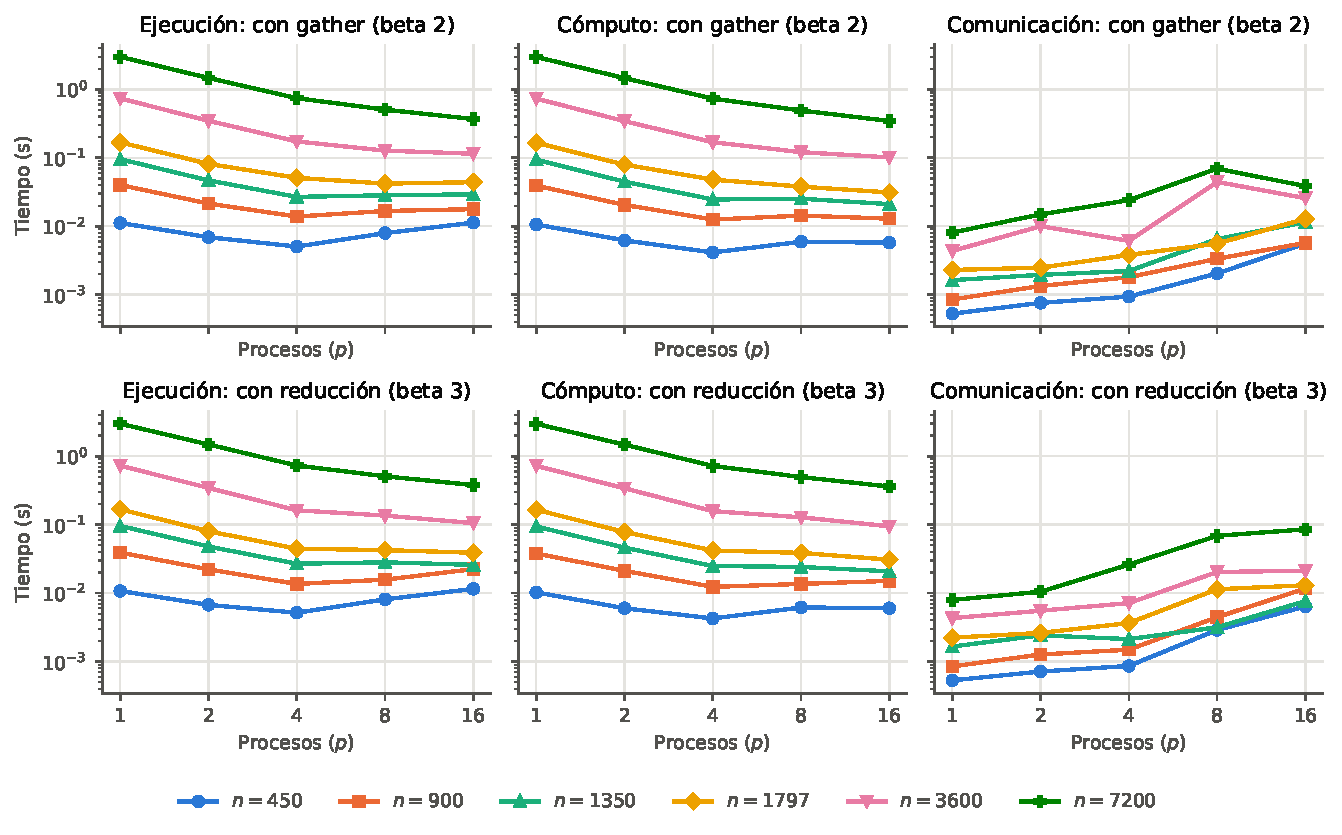
\includegraphics[width=\linewidth]{tiempos.pdf}
\caption{Tiempo de ejecución $T_p$, de cómputo ($\max_q t^{(q)}_{comp}$) y de comunicación (en el maestro) frente a $p$, para cada $n$. Arriba, con \texttt{Gather}; abajo, con la reducción.}
\label{fig:tiempos}
\end{figure}

\textbf{Ejecución.} Con $n\ge 3600$, $T_p$ baja hasta $p=16$: con $n=7200$, de 2,98\,s a 0,37\,s. Con $n\le 900$, el mínimo está en $p=4$ y después el tiempo sube: con $n=450$, pasa de 5,0\,ms en $p=4$ a 11,3\,ms en $p=16$. Con poco trabajo por proceso, el costo de agregar procesos supera la ganancia. Con $n=1350$ y $n=1797$ la curva queda casi plana desde $p=4$: con $n=1797$ y \texttt{Gather}, 51, 42 y 44\,ms en $p=4$, 8 y 16.

\textbf{Cómputo.} Hasta $p=4$ se reduce casi a la mitad cada vez que se duplica $p$. Por ejemplo, con $n=7200$ pasa de 2,98 a 1,46 y a 0,73\,s. De $p=4$ a $p=8$ solo baja 1,5 veces (0,49\,s), y de $p=8$ a $p=16$, 1,4 veces (0,34\,s). Es la limitación del hardware de la Sección~\ref{sec:entorno}: desde $p=8$ hay procesos en núcleos más lentos. En nuestras mediciones, este es el principal límite del \textit{speedup}, más que la comunicación.

El cómputo incluye el ordenamiento del paso 4, que resultó caro: con $p=1$ ocupa alrededor del 40\,\% del tiempo de las distancias más el ordenamiento (con $n=1797$, 70\,ms de 164\,ms). La Sección~\ref{sec:secuencial} supuso que el ordenamiento era menor porque $d>\log n$, y eso es cierto en cantidad de operaciones. Pero cada operación del ordenamiento cuesta mucho más que una suma o un producto vectorizados.

\textbf{Comunicación.} Crece con $p$ para todo $n$: con $n=1797$ y \texttt{Gather}, de 2,5\,ms en $p=2$ a 12,8\,ms en $p=16$. Con $p=1$ no es cero (2,3\,ms con $n=1797$), porque las colectivas en minúscula serializan los datos aunque haya un solo proceso \cite{mpi4py}; el Scatter solo ya toma 1,7\,ms. Algunos puntos son irregulares (con $n=3600$ y $p=8$, 44\,ms), porque la comunicación incluye la espera por los procesos más lentos.

\textbf{Granularidad.} La Figura~\ref{fig:granularidad} muestra $G=T_{comp}/T_{comm}$ \cite{slides}. Baja al aumentar $p$ y sube al aumentar $n$, como predice el modelo: el cómputo crece como $n^2$ y los datos enviados como $n$. $G$ es mayor que 1 en todas las configuraciones salvo $n=450$ con $p=16$, donde llega a 1 con \texttt{Gather} y baja apenas de 1 con la reducción. Es justamente donde el tiempo total ya subía.

\begin{figure}[ht]
\centering
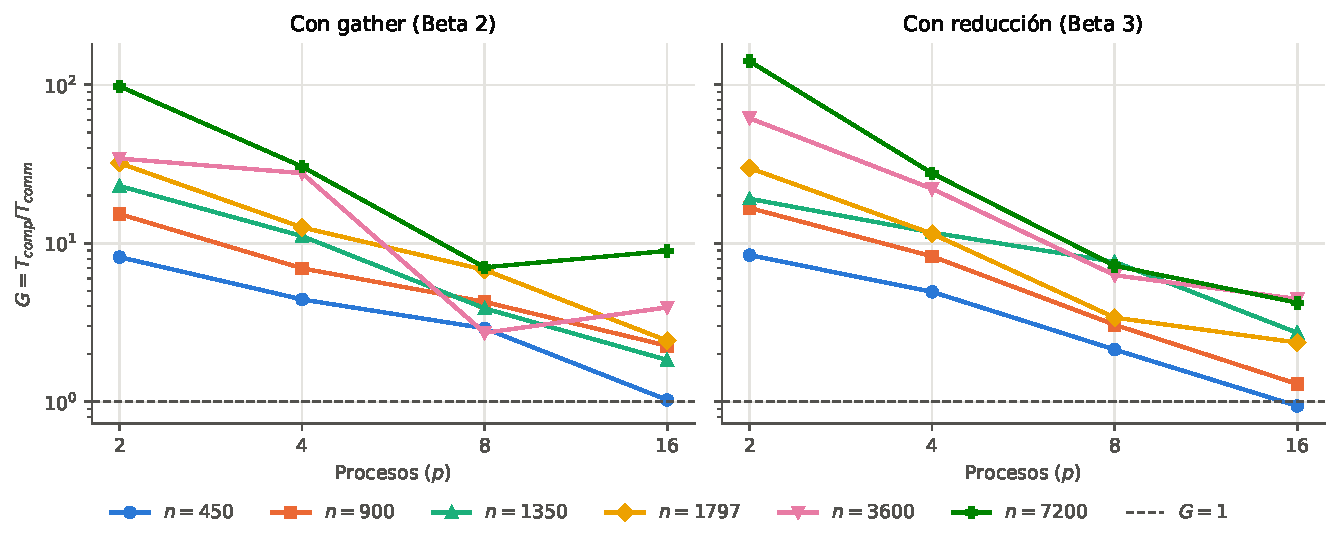
\includegraphics[width=0.92\linewidth]{granularidad.pdf}
\caption{Granularidad $G=T_{comp}/T_{comm}$. Con $G<1$ dominaría la comunicación.}
\label{fig:granularidad}
\end{figure}

\textbf{Precisión.} Con los datos originales y sus submuestras, la precisión es la misma para todo $p$ y para las dos versiones (Figura~\ref{fig:precision}): repartir el trabajo no cambia el resultado. Las diferencias entre valores de $n$ vienen de los conjuntos de prueba, que tienen 90, 180, 270 y 360 puntos, no del paralelismo.

\begin{figure}[ht]
\centering
\begin{minipage}{0.48\linewidth}
  \centering
  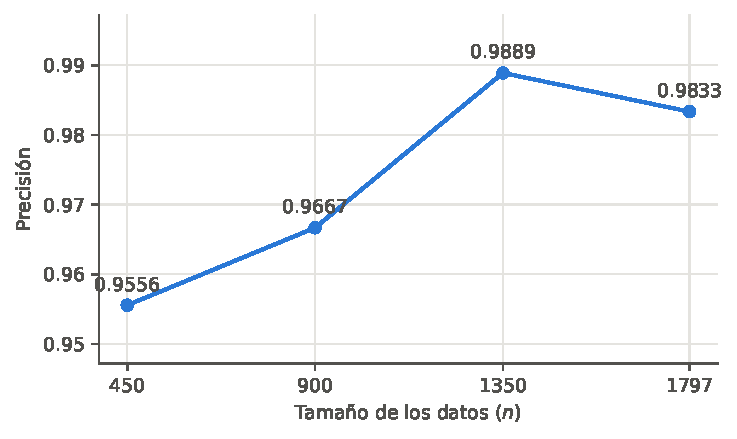
\includegraphics[width=\linewidth]{precision.pdf}
  \caption{Precisión frente a $n$ con los datos originales. Es la misma para todo $p$ y en las dos versiones.}
  \label{fig:precision}
\end{minipage}\hfill
\begin{minipage}{0.48\linewidth}
  \centering
  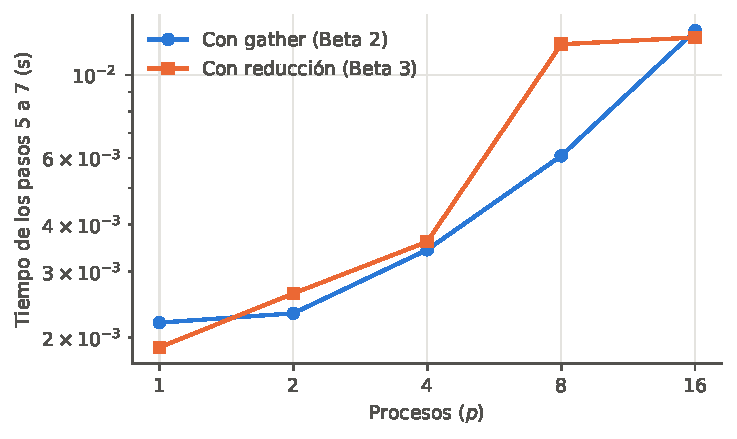
\includegraphics[width=\linewidth]{paso6.pdf}
  \caption{Tiempo de los pasos 5 a 7 (recolección, selección y votación) con $n=1797$.}
  \label{fig:paso6}
\end{minipage}
\end{figure}

\subsection{Comparación con la complejidad teórica}
\label{sec:normalizacion}

\textbf{Cómo se normalizó.} Para cada versión, ajustamos los coeficientes $c_i\ge 0$ de $\hat T$ (Sección~\ref{sec:metricas}) con las 30 medianas de $T_p$, por mínimos cuadrados no negativos. Minimizamos el error relativo, para que los tiempos de milisegundos pesen lo mismo que los de segundos. Cada $c_i$ está en segundos por unidad de su término, es decir, la expresión teórica se multiplica término a término por un costo medido. La Tabla~\ref{tab:coef} muestra los coeficientes y la Figura~\ref{fig:teoria} superpone $\hat T$ a las mediciones.

\begin{table}[ht]
\centering\small
\begin{tabular}{lccccc}
  \toprule
  \textbf{Versión} & $c_1$ (s) & $c_2$ (s) & $c_3$ (s) & $c_4$ (s) & \textbf{Error medio} \\
  \midrule
  \texttt{Gather} & $5{,}18\times10^{-8}$ & $1{,}12\times10^{-6}$ & $1{,}02\times10^{-7}$ & $4{,}01\times10^{-4}$ & 8,1\,\% \\
  Reducción & $4{,}87\times10^{-8}$ & --- & $3{,}95\times10^{-6}$ & $1{,}95\times10^{-4}$ & 11,5\,\% \\
  \bottomrule
\end{tabular}
\caption{Coeficientes de $\hat T(n,p)=c_1\,n^2/p+c_2\,n\,p+c_3\,n\log_2 p+c_4\log_2 p$ y error relativo medio del ajuste.}
\label{tab:coef}
\end{table}

\begin{figure}[ht]
\centering
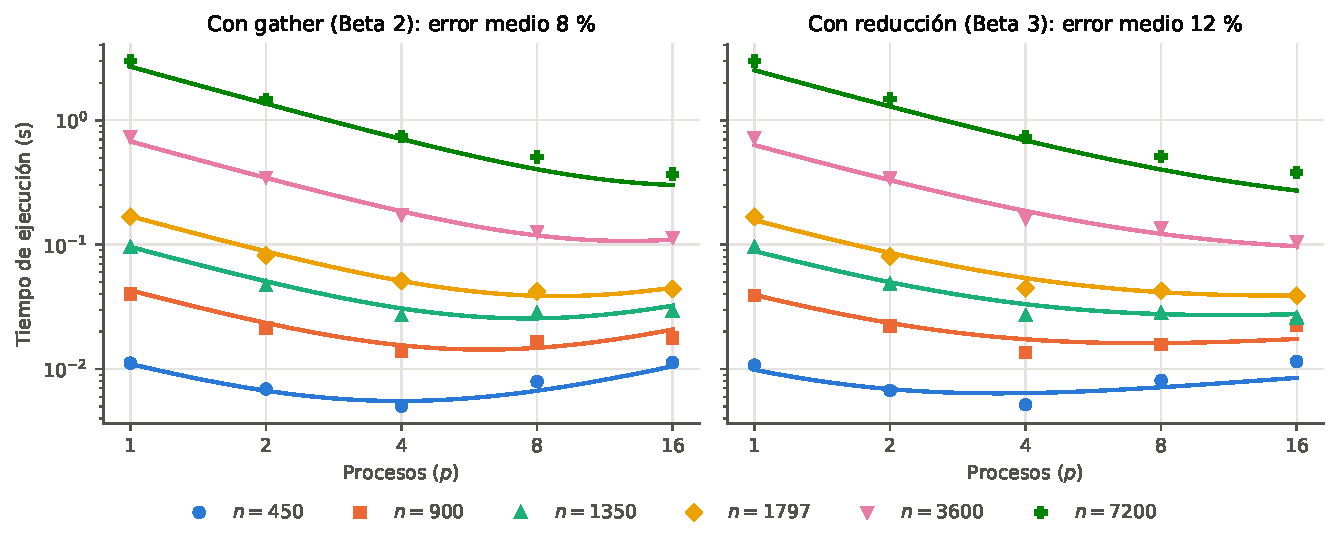
\includegraphics[width=0.92\linewidth]{teoria.pdf}
\caption{Tiempo de ejecución medido (puntos) y modelo normalizado $\hat T$ (líneas).}
\label{fig:teoria}
\end{figure}

\textbf{Significado de cada coeficiente.}
\begin{itemize}
  \item $c_1$: como $\ntr\,\nte\approx 0{,}16\,n^2$, equivale a $3{,}2\times10^{-7}$\,s por distancia, incluida su parte del ordenamiento. Dividido entre los $3d=192$ FLOP de una distancia, son $1{,}7\times10^{-9}$\,s por FLOP, es decir 0,59\,GFLOP/s. Es lo que se mide con $p=1$: entre 0,53 y 0,64\,GFLOP/s (Figura~\ref{fig:flops}).
  \item $c_3$: el término de datos dominante es el del Broadcast, con $\nte\,d=12{,}8\,n$ datos. Con el $b$ del ping-pong, el modelo predice $12{,}8\,b=7{,}5\times10^{-8}$\,s. El ajuste da $1{,}0\times10^{-7}$\,s, del mismo orden.
  \item $c_4$: con tres colectivas que pagan $a\log p$ cada una, el modelo predice $3a=1{,}1\times10^{-4}$\,s. El ajuste da 3,7 veces más, porque $c_4$ absorbe todo lo que crece como $\log p$ y no está modelado: la serialización y la espera por los procesos lentos. En cambio, al ajustar solo $T_{comm}$, el coeficiente de latencia es $3{,}5\times10^{-5}$\,s, prácticamente el $a$ del ping-pong ($3{,}6\times10^{-5}$\,s).
  \item $c_2$: debería ser el costo de la selección en el maestro. Pero la selección medida con $n=1797$ y $p=16$ toma 4,7\,ms, lo que da unos $1{,}6\times10^{-7}$\,s por unidad de $n\,p$: el ajuste da 7 veces más. $c_2$ absorbe todo lo que crece linealmente con $p$, sobre todo el cómputo que deja de escalar desde $p=8$.
  \item En la reducción, $c_3$ es 40 veces mayor que con \texttt{Gather}. En $\hat T'$, el término de las fusiones $\oplus$, $k\,n\log p$, y el de datos comparten la misma columna $n\log p$. Así que $c_3$ mide sobre todo las fusiones, que se hacen en Python por cada punto de prueba.
\end{itemize}

\textbf{Error.} El modelo reproduce la forma de las curvas, con su mínimo, y tiene un error medio de 8\,\% con \texttt{Gather} y 12\,\% con la reducción. Las mayores desviaciones están en $p=8$ con $n$ grande: con $n=7200$, el modelo da 0,40\,s y se midió 0,51\,s. Es el punto en que entran los núcleos de eficiencia.

\textbf{Cómputo y comunicación por separado.} La Figura~\ref{fig:fases} ajusta cada fase con sus propios términos. El cómputo tiene un error de 10 a 11\,\%. La comunicación tiene un error de 28 a 35\,\%: son tiempos de milisegundos, con ruido, y que incluyen esperas. En el ajuste de la comunicación con \texttt{Gather} agregamos el término $n(p-1)$ del modelo de árbol binomial \cite{thakur}, y su coeficiente no es nulo ($1{,}8\times10^{-7}$\,s). Es decir, la comunicación medida crece más rápido que $\log p$, como anticipamos en la Sección~\ref{sec:metricas}: el maestro recibe físicamente $p-1$ bloques. La forma $\log p$ del curso describe bien la latencia, pero es una cota inferior para el término de datos del \texttt{gather}.

\begin{figure}[ht]
\centering
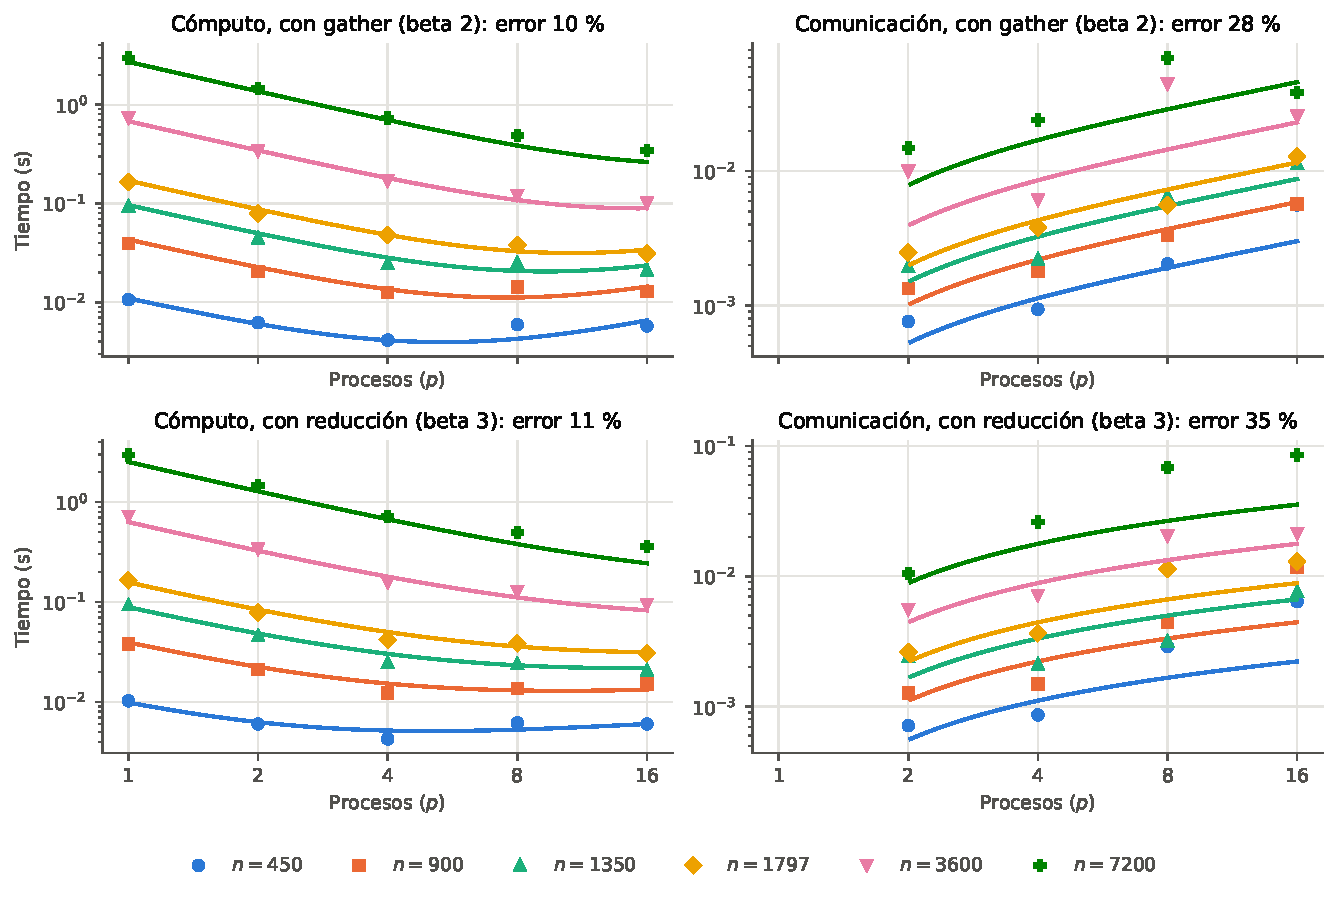
\includegraphics[width=0.92\linewidth]{teoria_fases.pdf}
\caption{Cómputo y comunicación medidos (puntos) y su ajuste por separado (líneas).}
\label{fig:fases}
\end{figure}

\subsection{Número óptimo de procesos}
\label{sec:optimo}

La Tabla~\ref{tab:optimo} compara $p^*$, calculado con los coeficientes de la Tabla~\ref{tab:coef}, con el $p$ de menor tiempo medido.

\begin{table}[ht]
\centering\small
\begin{tabular}{rcccc}
  \toprule
  & \multicolumn{2}{c}{\textbf{Con \texttt{Gather}}} & \multicolumn{2}{c}{\textbf{Con reducción}} \\
  \cmidrule(lr){2-3}\cmidrule(lr){4-5}
  $n$ & $p^*$ estimado & mejor $p$ medido & $p^{*\prime}$ estimado & mejor $p$ medido \\
  \midrule
  450  & 4,6  & 4  & 3,5  & 4 \\
  900  & 6,4  & 4  & 7,3  & 4 \\
  1350 & 7,9  & 4  & 11,1 & 16 \\
  1797 & 9,1  & 8  & 15,0 & 16 \\
  3600 & 12,9 & 16 & 30,4 & 16 \\
  7200 & 18,2 & 16 & 61,2 & 16 \\
  \bottomrule
\end{tabular}
\caption{Número óptimo de procesos estimado con el modelo y mejor $p$ de la malla medida.}
\label{tab:optimo}
\end{table}

Con \texttt{Gather}, $p^*=\sqrt{c_1 n/c_2}$ crece como $\sqrt{n}$. Coincide con el mejor $p$ medido, dentro de la resolución de la malla (potencias de 2), para $n=450$ y para $n\ge 1797$. Para $n=900$ y $n=1350$ lo sobrestima, pero allí el mínimo es plano: con $n=1350$, $p=4$ y $p=8$ difieren en un 6\,\% (26,8 frente a 28,3\,ms). Con la reducción, $p^{*\prime}$ crece casi como $n$. Para $n\ge 1797$ queda en el borde de la malla o fuera de ella, lo que coincide con que el mejor $p$ medido sea 16, pero no se puede verificar sin más núcleos. En ambos casos $\hat T''(p^*)>0$, así que son mínimos.

\textbf{Para el conjunto original ($n=1797$), el número óptimo de procesos es $p=8$}: el modelo da 9,1 y la medición, 8.

Las curvas de cómputo y comunicación no se cruzan en este rango (Figura~\ref{fig:tiempos}): la comunicación medida queda por debajo del cómputo, salvo con $n=450$ y $p=16$, donde se igualan. Así que, aquí, el criterio del cruce \cite{slides} solo marca el límite para el $n$ más pequeño. Para el resto, el óptimo lo fijan el costo que crece con $p$ en el maestro y la limitación del hardware.

\subsection{\textit{Speedup} y FLOPs}
\label{sec:speedup}

\textbf{$T_s$ y código base.} Para $n\ge 900$, $T_s$ difiere en menos de 3\,\% de la corrida con $p=1$ (con $n=1797$, 0,166 frente a 0,168\,s), así que el costo de MPI con un proceso es pequeño. Con $n=450$ la diferencia es de 9\,\%, porque el tiempo total es de solo 10\,ms. El código base \cite{base} tarda 3,42\,s con $n=1797$, 20,6 veces más que $T_s$: eso es lo que aporta la vectorización. Juntando ambas cosas, la mejor versión paralela es entre 80 y 90 veces más rápida que el código base, pero de ese factor el paralelismo aporta solo unas 4 veces. Por eso el \textit{speedup} se mide contra $T_s$ y no contra el código base.

\begin{figure}[ht]
\centering
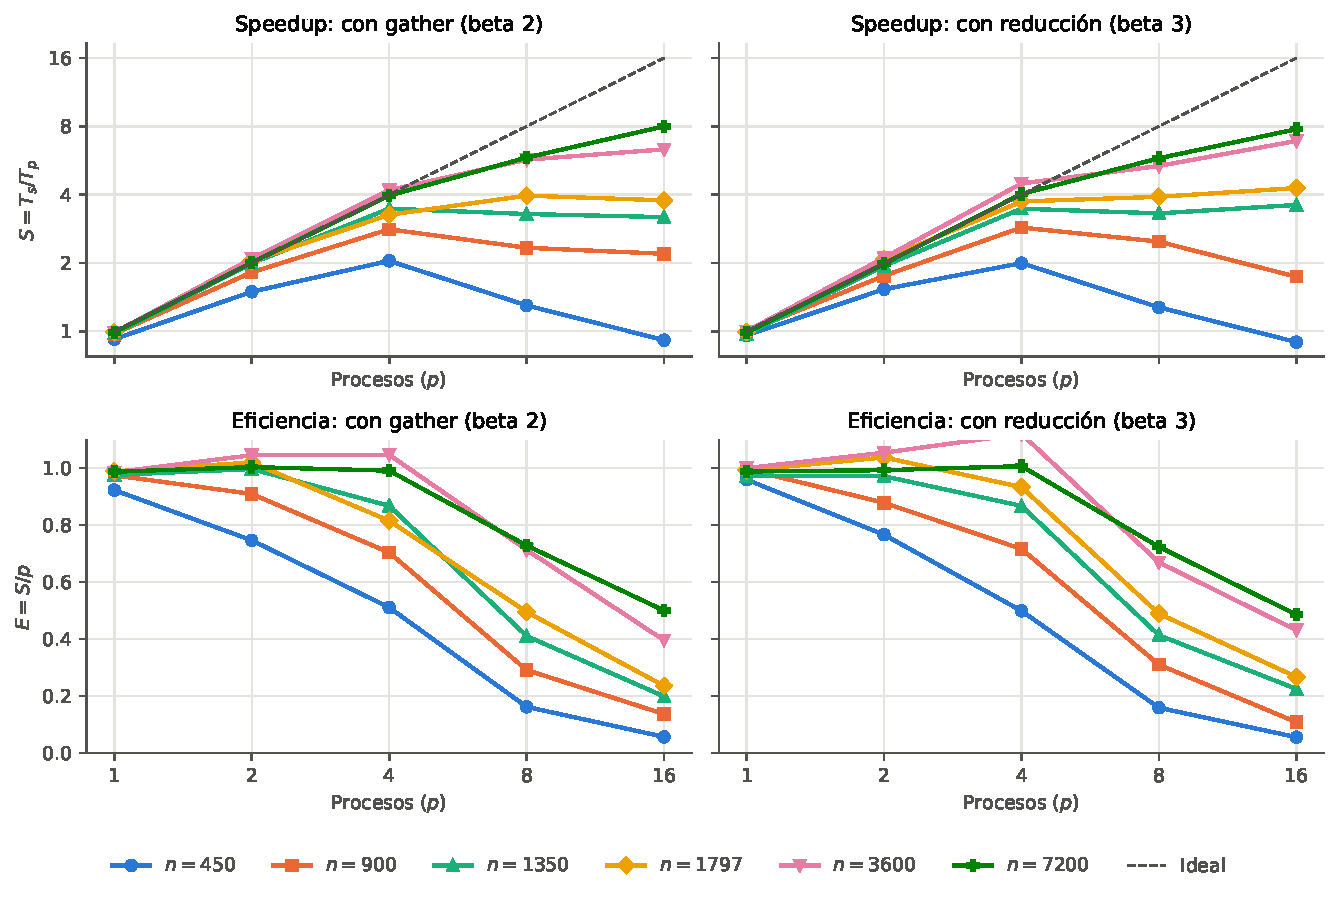
\includegraphics[width=0.92\linewidth]{speedup_eficiencia.pdf}
\caption{\textit{Speedup} $S=T_s/T_p$ (arriba, escala logarítmica) y eficiencia $E=S/p$ (abajo). La línea punteada es el \textit{speedup} ideal.}
\label{fig:speedup}
\end{figure}

\textbf{\textit{Speedup}.} La Figura~\ref{fig:speedup} muestra que es casi lineal hasta $p=4$ para $n\ge 1350$. El máximo es 8,00 con \texttt{Gather} y 7,77 con la reducción, ambos con $n=7200$ y $p=16$. Con los datos originales ($n=1797$) llega a 3,96 en $p=8$ con \texttt{Gather} y a 4,28 en $p=16$ con la reducción. Con $n=3600$ y $p=2$ a 4, la eficiencia supera ligeramente 1 (hasta 1,05 con \texttt{Gather} y 1,12 con la reducción). Probablemente es un efecto de caché, porque los bloques más pequeños caben mejor en ella; no lo verificamos. No es el error de la Sección~\ref{sec:betas}, que daba un factor de 4 y ya está corregido.

\textbf{FLOPs.} La Figura~\ref{fig:flops} muestra $F/T_p$ y $F/\max_q t^{(q)}_{comp}$. Como $F$ no depende de $p$, $F/T_p$ sigue la forma del \textit{speedup}: de 0,53 a 0,64\,GFLOP/s con $p=1$ hasta 4,33\,GFLOP/s con \texttt{Gather} y 4,20 con la reducción ($n=7200$, $p=16$). Con $n=1797$ el máximo es 2,37\,GFLOP/s, en $p=8$. Si se excluye la comunicación, con $n=7200$ y $p=16$ se llega a 4,9\,GFLOP/s. Estos valores subestiman el trabajo real, porque $F$ solo cuenta las distancias y no el ordenamiento.

\begin{figure}[ht]
\centering
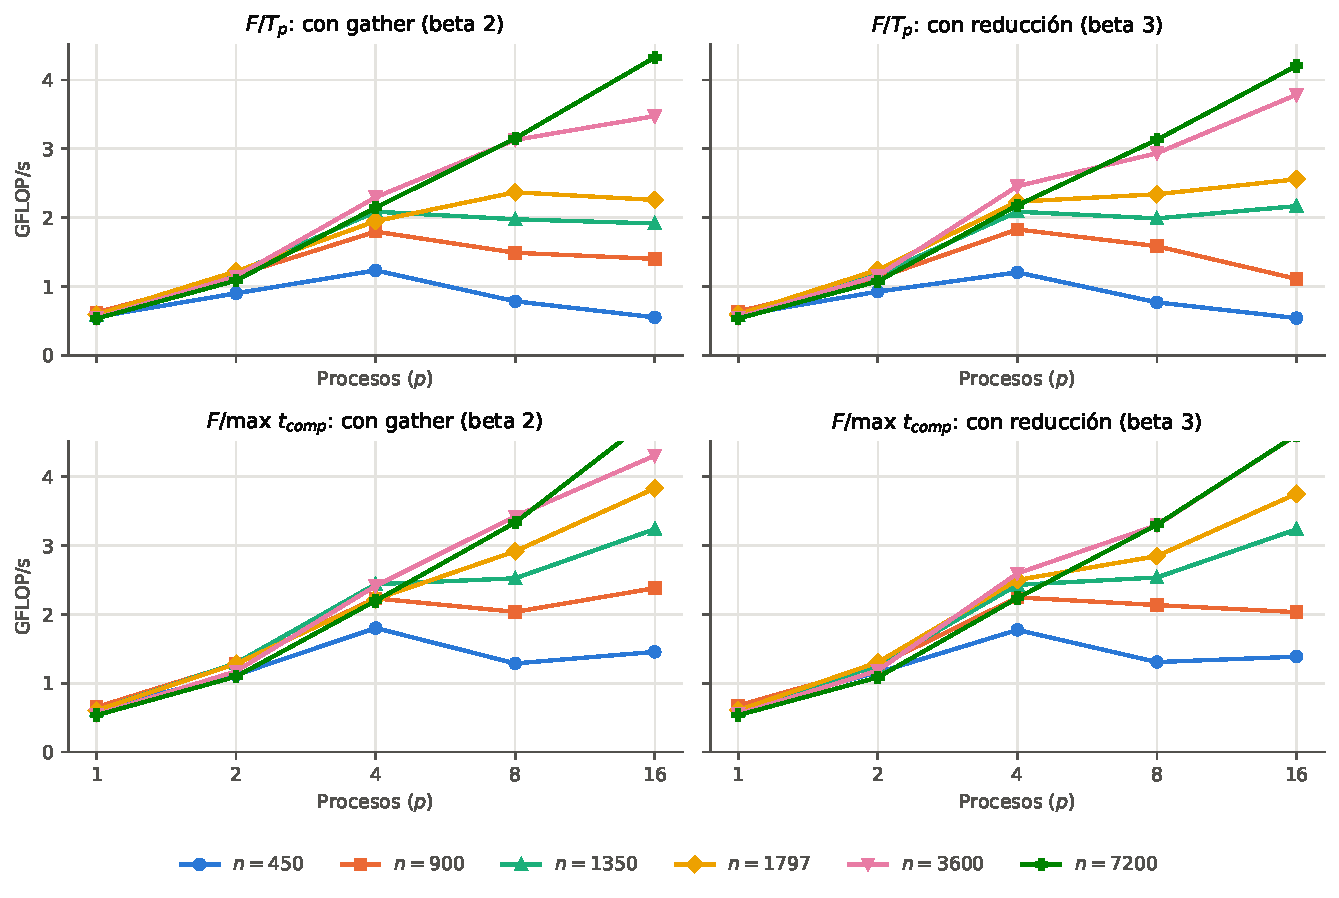
\includegraphics[width=0.92\linewidth]{flops.pdf}
\caption{FLOP por segundo en la región paralelizable, con el tiempo total (arriba) y solo con el de cómputo (abajo).}
\label{fig:flops}
\end{figure}

\subsection{Escalabilidad}
\label{sec:escalabilidad}

\textbf{Eficiencia con $n$ variable.} En la Figura~\ref{fig:speedup} (abajo), la eficiencia baja al aumentar $p$ y sube al aumentar $n$. Con $p=16$ va de 0,06 con $n=450$ a 0,50 con $n=7200$. El algoritmo solo mantiene su eficiencia si el problema crece junto con $p$, como predice $E=O\big(1/(1+p^2/n)\big)$.

\textbf{Validación de la isoeficiencia.} Seguimos el método del curso \cite{slides}: escalar $n$ según la condición y comprobar si $E$ se mantiene. Medimos dos series de pares $(n,p)$, con $n/p^2\approx 28$ y con $n/(p\log_2 p)\approx 56$. Cada serie sirve además de control para la otra versión. La Tabla~\ref{tab:iso} y la Figura~\ref{fig:iso} comparan la $E$ medida con la que predice el modelo normalizado, $\hat E=\hat T(n,1)/(p\,\hat T(n,p))$.

\begin{table}[ht]
\centering\small
\begin{tabular}{llcccc}
  \toprule
  & & \multicolumn{2}{c}{\textbf{Con \texttt{Gather}}} & \multicolumn{2}{c}{\textbf{Con reducción}} \\
  \cmidrule(lr){3-4}\cmidrule(lr){5-6}
  \textbf{Condición} & $(n,p)$ & $E$ medida & $\hat E$ & $E$ medida & $\hat E$ \\
  \midrule
  $n\propto p^2$ & (450, 4)  & 0,511 & 0,496 & 0,499 & 0,385 \\
                 & (1797, 8) & 0,495 & 0,545 & 0,489 & 0,474 \\
                 & (7200, 16)& 0,500 & 0,558 & 0,486 & 0,580 \\
  \midrule
  $n\propto p\log_2 p$ & (450, 4)  & 0,511 & 0,496 & 0,499 & 0,385 \\
                       & (1350, 8) & 0,411 & 0,469 & 0,413 & 0,401 \\
                       & (3600, 16)& 0,396 & 0,385 & 0,431 & 0,407 \\
  \bottomrule
\end{tabular}
\caption{Eficiencia medida y del modelo normalizado en las series de isoeficiencia.}
\label{tab:iso}
\end{table}

\begin{figure}[ht]
\centering
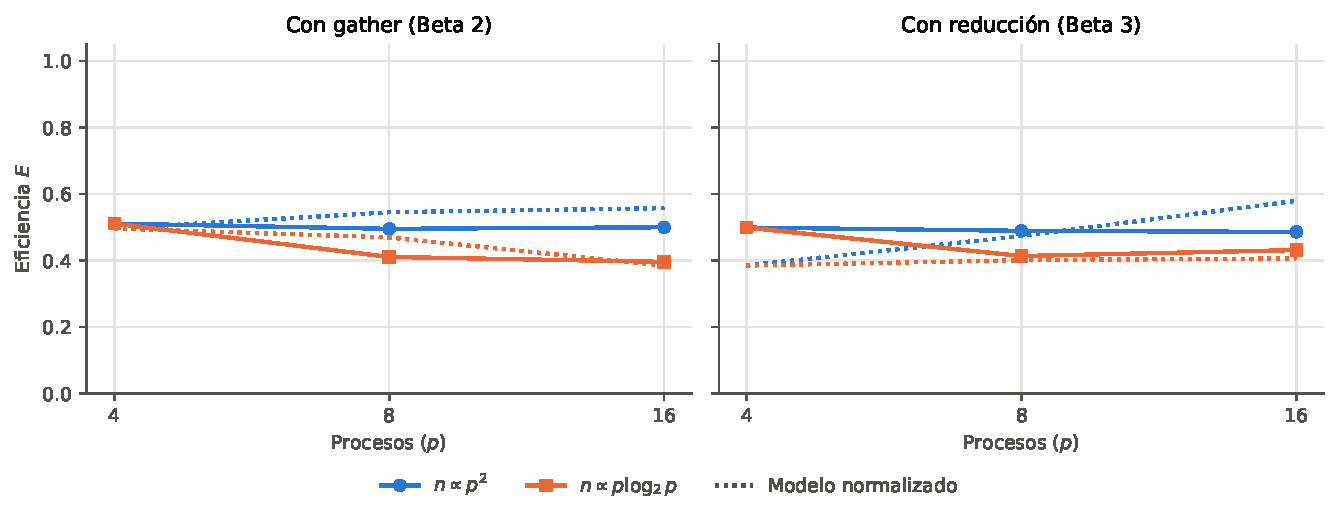
\includegraphics[width=0.92\linewidth]{isoeficiencia.pdf}
\caption{Eficiencia en las series de isoeficiencia. Línea continua: medida; punteada: modelo normalizado.}
\label{fig:iso}
\end{figure}

\begin{itemize}
  \item \textbf{\texttt{Gather}, condición $n\propto p^2$: se cumple.} $E$ se mantiene en 0,51, 0,50 y 0,50 mientras $p$ pasa de 4 a 16, con una variación de unos 3\,\%. Esto valida con los datos la condición $n=\Omega(p^2)$ de la Sección~\ref{sec:metricas}.
  \item \textbf{\texttt{Gather}, control con $n\propto p\log p$: $E$ cae} de 0,51 a 0,41 y a 0,40. Hacer crecer $n$ más lento que $p^2$ no alcanza para esta versión, como predice el modelo.
  \item \textbf{Reducción, condición $n\propto p\log p$: no se cumple del todo.} $E$ baja de 0,50 a 0,41 y sube a 0,43, una caída de 14 a 17\,\%. Con $n\propto p^2$ se mantiene (0,50, 0,49 y 0,49). La reducción elimina el término $k\,n\,p$ de la selección en el maestro, pero ese término medido es pequeño (la selección toma menos de 5\,ms con $n=1797$ y $p=16$). La pérdida de eficiencia viene, sobre todo, del cómputo que deja de escalar desde $p=8$ (Sección~\ref{sec:tiempos}). Ese efecto afecta igual a las dos versiones y crece más rápido que $p\log p$. Por eso, en este rango, la reducción no muestra la mejor escalabilidad que predice la teoría.
\end{itemize}

El modelo normalizado sigue las series medidas con una diferencia de hasta 0,06 con \texttt{Gather} y de hasta 0,11 con la reducción. Dos advertencias: las condiciones de isoeficiencia son asintóticas, y cada serie tiene solo tres puntos, hasta $p=16$. Además, con $p=16$ hay más procesos que núcleos físicos. Para separar el algoritmo del hardware habría que repetir estas series en una máquina con al menos 16 núcleos iguales, como Khipu o las PC del laboratorio L507.

\subsection{Mejoras a la solución}
\label{sec:mejoras}

\textbf{\texttt{Gather} frente a la reducción.} La mejora que implementamos (Algoritmo~\ref{alg:knnred}) no da una ganancia clara en las mediciones. Los tiempos totales de las dos versiones difieren poco y en ambas direcciones. Con $n=1797$ y $p=16$ gana la reducción (\textit{speedup} de 4,28 frente a 3,77). Con $n=900$ y $p=16$ gana \texttt{Gather} (2,19 frente a 1,74). La Figura~\ref{fig:paso6} muestra los pasos 5 a 7 con $n=1797$: en ambas versiones pasan de unos 2\,ms con $p=1$ a 13\,ms con $p=16$, y con $p=8$ la reducción es más lenta (12 frente a 6\,ms). La razón es que, con $p\le 16$ y $k=3$, el maestro revisa a lo más 48 candidatos por punto de prueba, así que la reducción ahorra poco. A cambio, cada nivel del árbol serializa objetos y ejecuta $\oplus$ en Python. Esto coincide con lo que anticipó el profesor: el ahorro es pequeño \cite{correo-profesor}. La reducción convendría con muchos más procesos o con un $k$ mayor.

Otras mejoras que se desprenden de las mediciones:
\begin{itemize}
  \item \textbf{Ordenamiento parcial en el paso 4.} El ordenamiento ocupa alrededor del 40\,\% del cómputo con $p=1$ (Sección~\ref{sec:tiempos}). Con \texttt{np.argpartition} se obtienen los $k$ menores en tiempo lineal, sin ordenar todo el bloque. Esto reduce $\tcomp{1}$, aunque cambia el término $\log(\ntr/p)$ de la Tabla~\ref{tab:costos}.
  \item \textbf{Colectivas con arreglos de NumPy.} Las funciones en mayúscula de mpi4py (\texttt{Bcast}, \texttt{Scatterv}, \texttt{Gather}) envían los arreglos sin serializarlos \cite{mpi4py}. Esto bajaría la latencia medida, que hoy está dominada por la serialización, y la comunicación con $p=1$. \texttt{Scatterv} permite bloques de distinto tamaño.
  \item \textbf{Reparto según la velocidad de cada núcleo.} Con núcleos de dos tipos, bloques iguales no equivalen a carga balanceada. Se puede fijar cada proceso a un núcleo, o dar bloques más grandes a los núcleos de rendimiento.
  \item \textbf{Ejecución en un clúster.} Medir en Khipu o en el laboratorio L507, con núcleos iguales y más de 16, permitiría verificar $p^{*\prime}$ y la isoeficiencia de la reducción.
  \item \textbf{Versión híbrida.} Combinar MPI entre nodos con hilos dentro de cada nodo. No la implementamos, porque el enunciado pide memoria distribuida.
\end{itemize}

% ---------------------------------------------------------------- Bibliografía
\renewcommand{\refname}{Bibliografía}
\begin{thebibliography}{9}
\setlength{\itemsep}{3pt}

\bibitem{enunciado} J. Fiestas, \textit{Computación Paralela y Distribuida: Proyecto -- Laboratorio}, 2026-II. Lima, Perú: UTEC, 2026.\\
\textbf{Impacto:} define el caso 5 y el contenido del informe. De aquí tomamos el DAG (Figura~\ref{fig:dag}) y la distribución de datos de la Introducción (\textit{broadcast} de prueba, \textit{scatter} de entrenamiento, \textit{gather} de candidatos).

\bibitem{base} \texttt{knn\_digits\_sec.py}, código secuencial del caso 5, adjunto al enunciado \cite{enunciado}. [Online]. Available: \url{https://drive.google.com/file/d/1wTBSh7bwT1QVvce0pFMv5tcCWsg4-HeK/view} (accessed Sep. 18, 2026).\\
\textbf{Impacto:} es el código que paralelizamos. De él obtuvimos $T_s$ (Sección~\ref{sec:secuencial}), los parámetros ($k=3$, división 80/20, \texttt{random\_state=42}) y la precisión de referencia ($0{,}9833$).

\bibitem{mpi4py} L. Dalcin, \textit{MPI for Python (mpi4py) documentation} [Online]. Available: \url{https://mpi4py.readthedocs.io/en/stable/} (accessed Nov. 4, 2026).\\
\textbf{Impacto:} revisamos cómo funcionan \texttt{comm.bcast}, \texttt{comm.scatter} y \texttt{comm.gather}, y que las reducciones de objetos usan un árbol por defecto (\texttt{mpi4py.rc.fast\_reduce}), lo que sustenta el Algoritmo~\ref{alg:knnred}. También explica que las funciones en minúscula serializan los objetos, lo que usamos para interpretar la latencia medida y la comunicación con $p=1$ (Secciones~\ref{sec:entorno} y~\ref{sec:tiempos}), y para proponer las colectivas con arreglos de NumPy (Sección~\ref{sec:mejoras}).

\bibitem{sklearn} F. Pedregosa \textit{et al.}, ``Scikit-learn: Machine Learning in Python,'' \textit{Journal of Machine Learning Research}, vol. 12, pp. 2825--2830, 2011.\\
\textbf{Impacto:} es la librería que usa el código base (\texttt{load\_digits}, \texttt{train\_test\_split}). De ella salen los datos y su división, descritos en la Introducción.

\bibitem{slides} J. Fiestas, diapositivas y apuntes del curso CS4052: U1.1 Fundamentos de paralelismo, U1.2 Fundamentos (Foster, Flynn), U1.3 DAG, U2.1 Diseño en paralelo (\textit{performance}), U2.2 PRAM 01, U2.3 PRAM 02, U2.4 Particionamiento, U3.2, U3.5, U6.1 y U6.2 (\textit{performance}). Lima, Perú: UTEC, 2026.\\
\textbf{Impacto:} son la base teórica del informe: paralelización natural (Introducción), pasos de Foster y particiones balanceadas (Sección~\ref{sec:foster}), formato del PRAM con \textbf{pardo}, pasos numerados y CREW (Sección~\ref{sec:pram}), teorema de Brent (Sección~\ref{sec:span}), y $S=T_s/T_p$, $E=S/p$, isoeficiencia, FLOPs, medición de $a$ y $b$ y el modelo $T_{comm}=f(p)(\alpha+x\beta)$ (Sección~\ref{sec:metricas}). En los resultados seguimos su ping-pong para medir $a$ y $b$ (Sección~\ref{sec:entorno}), la granularidad $G$ y el cruce de cómputo y comunicación (Secciones~\ref{sec:tiempos} y~\ref{sec:optimo}), y su método para validar la isoeficiencia escalando $n$ (Sección~\ref{sec:escalabilidad}).

\bibitem{pd02} J. Fiestas, \textit{CS4052 -- Práctica Dirigida 02 (solución)}. Lima, Perú: UTEC, 2026.\\
\textbf{Impacto:} nos sirvió de modelo para escribir el pseudocódigo con Scatter, Broadcast y Gather (Sección~\ref{sec:pram}) y para expresar la eficiencia en la forma $E=O(1/(1+\dots))$ (Sección~\ref{sec:metricas}).

\bibitem{thakur} R. Thakur, R. Rabenseifner y W. Gropp, ``Optimization of Collective Communication Operations in MPICH,'' \textit{International Journal of High Performance Computing Applications}, vol. 19, no. 1, pp. 49--66, 2005.\\
\textbf{Impacto:} describe el modelo de árbol binomial para las colectivas, que comentamos en la Sección~\ref{sec:metricas} como explicación física de por qué el maestro recibe $(p-1)$ bloques en el \textit{gather}. En la Sección~\ref{sec:normalizacion} usamos su término $n(p-1)$ para ajustar la comunicación medida.

\bibitem{correo-profesor} J. Fiestas, respuesta por correo electrónico a consulta del grupo sobre el costo de \texttt{scatter} y \texttt{gather} y el acceso a Khipu, 6 de noviembre de 2026 (comunicación personal).\\
\textbf{Impacto:} confirma que el costo correcto es $O(\log p)$ y no $O(p)$, lo que sustenta la Sección~\ref{sec:metricas}, la Tabla~\ref{tab:costos} y la Figura~\ref{fig:dag}. También autorizó medir en una laptop (Sección~\ref{sec:entorno}) y anticipó que la reducción ahorraría poco, lo que contrastamos con las mediciones (Sección~\ref{sec:mejoras}).

\bibitem{numpy} C. R. Harris \textit{et al.}, ``Array programming with NumPy,'' \textit{Nature}, vol. 585, pp. 357--362, 2020.\\
\textbf{Impacto:} es la librería con la que se calculan las distancias en el código paralelo. Su manejo de arreglos temporales explicó el problema de rendimiento descrito en la Sección~\ref{sec:betas}.

\bibitem{ia} Anthropic, \textit{Claude Opus 5}, \textit{Claude Sonnet 5} y \textit{Claude Opus 5.5} (asistentes de inteligencia artificial, usados con Claude Code), setiembre y noviembre de 2026.\\
\textbf{Uso:} en la entrega parcial, resumió y ordenó el material de clase y redactó el borrador del informe. En esta entrega:
\begin{itemize}
  \item Redactó en LaTeX la versión corregida del Método según las observaciones del profesor: pseudocódigo y diagramas (Secciones~\ref{sec:foster} y~\ref{sec:pram}), trabajo y \textit{span} (Sección~\ref{sec:span}) y métricas (Sección~\ref{sec:metricas}). Después aplicó la corrección de \textit{scatter} y \textit{gather} a $O(\log p)$ que confirmó el profesor \cite{correo-profesor}.
  \item Escribió el código de las versiones beta y los scripts de validación, experimentos y gráficas. Detectó los problemas de medición de la Sección~\ref{sec:betas}, incluido el de la ejecución que se colgó.
  \item Comparó el Método con las diapositivas del curso \cite{slides}.
  \item Redactó la sección de Resultados a partir de las mediciones y de los coeficientes calculados por los scripts, y armó la presentación final.
\end{itemize}
Cada cifra de los Resultados se contrastó con los archivos de mediciones. Las mediciones las ejecutó el grupo en su laptop.\\
\textbf{Impacto:} la mayor parte de la redacción y del código se hizo con esta herramienta, lo que ahorró tiempo. También propuso la reducción en árbol para optimizar el paso 6 (Algoritmo~\ref{alg:knnred}). El grupo es responsable de lo presentado.

\end{thebibliography}

\end{document}
